% !TEX encoding = UTF-8
% !TEX TS-program = pdflatex
% !TEX root = ../../tesi.tex

\section{L'azienda Sync Lab}
Sync Lab nasce come \textit{software house} nel 2002, per poi crescere rapidamente nel mercato del \gls{ICT}. In seguito ad una maturazione delle competenze tecnologiche, metodologiche ed applicative nel dominio del \textit{software}, si è tramutata in \gls{System Integrator} conquistando significative fette di mercato nei settori: \textit{mobile}, videosorveglianza e sicurezza delle infrastrutture informatiche aziendali. Attualmente possiede più di 150 clienti diretti e finali, 200 dipendenti e 5 sedi distribuite in tutta Italia. 

\begin{figure}[!h]
  \centering
  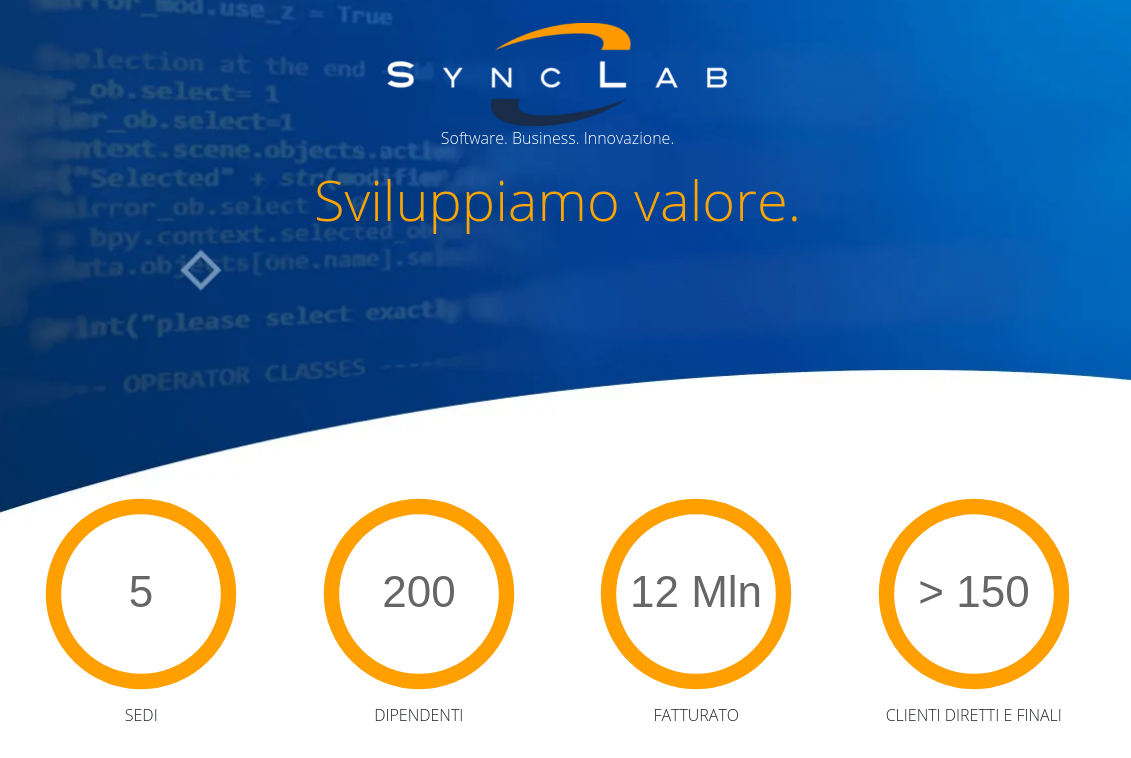
\includegraphics[width=\textwidth]{capitolo1/motto-synclab.png}
  \caption{Motto di Sync Lab e le sue statistiche}
  \textbf{Fonte}: \href{https://www.synclab.it}{https://www.synclab.it}
\end{figure}

Sync Lab consegue l'obiettivo principale di supportare il cliente nella realizzazione, messa in opera e controllo di soluzioni \textit{IT}, sia dal punto di vista tecnologico, sia nel governo del cambiamento organizzativo. Nel corso degli anni ha aumentato la propria qualità organizzativa e produttiva, riuscendo ad acquisire le seguenti 4 certificazioni: ISO 9001, ISO 14001, ISO 27001 e ISO 45001.



